\documentclass[12,border=3pt,tikz]{standalone}
\usepackage{amsmath}
\usepackage{enumerate}
\usepackage{tikz}
\usepackage{xcolor}
\usepackage{tikz-3dplot}
\usepackage{hyperref}
\usepackage{ifthen}
\usepackage{pgfplots}
\pgfplotsset{compat=1.11,
  colormap={myblue}{  rgb255(0cm)=(0,0,120)   rgb255(1cm)=(0,0,255)},
  colormap={myyellow}{rgb255(0cm)=(170,170,0) rgb255(1cm)=(255,255,0)}}

\begin{document}
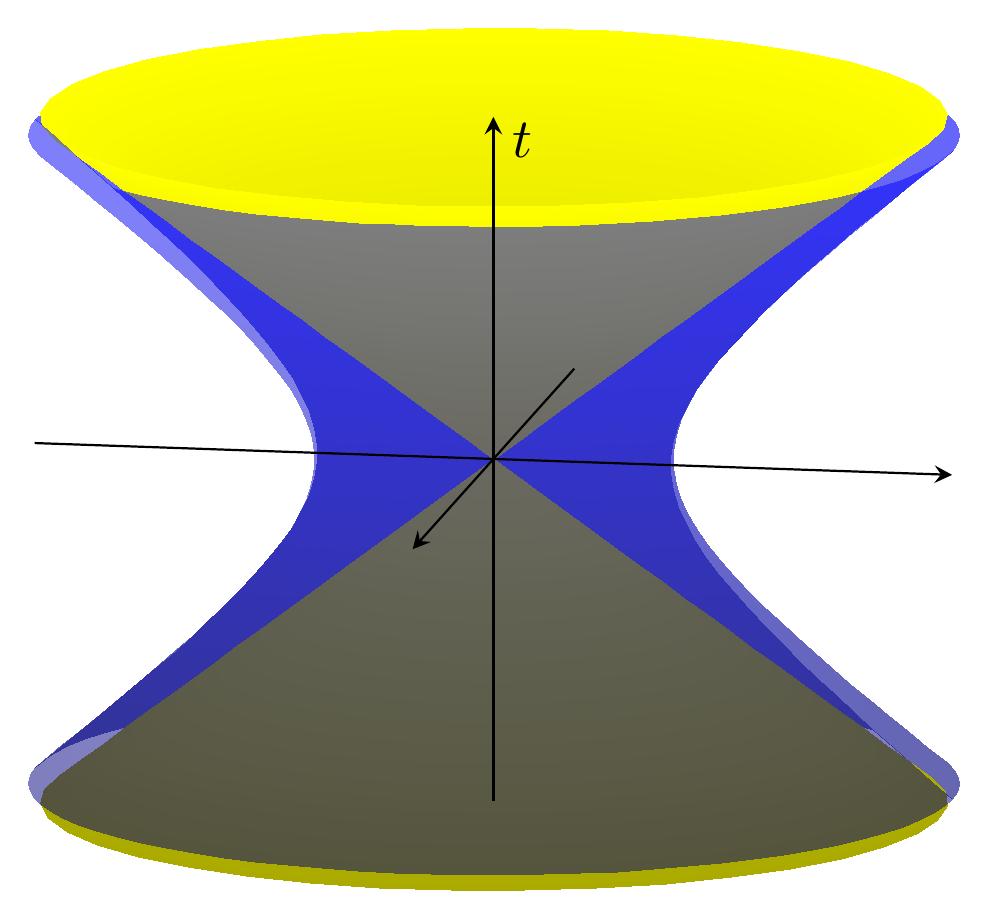
\begin{tikzpicture}[scale=2]
\begin{axis}[samples=40,axis lines=center,axis on top,view={100}{15},
             zlabel={$t$},%xlabel={$x$}, ylabel={$y$},
	         xtick=\empty,ytick=\empty,ztick=\empty]
	% https://tex.stackexchange.com/questions/39889/tikz-how-to-get-a-few-smooth-grid-lines-for-surface-plots
    \def\r{1.5}
    \def\h{4}
    \def\hs{3.6}
    \def\c{3.8}
    \def\w{1.1}
    \def\redge{100} % angle
    \def\ledge{180+\redge} % angle
    % patch,patch type=triangle quadr,domain=-2:2,shader=faceted interp,colormap/gray,fill=black, color=red,surf
    \addplot3[domain=-\hs:\hs,y domain=90:270,z buffer=sort,surf,
              colormap name={myblue},shader=interp,fill opacity=0.60]
             ({sqrt(x^2+\r^2)*cos(y)},{sqrt(x^2+\r^2)*sin(y)},x); % spacetime hyperboloid
    \addplot3[domain=-\c:\c,y domain=0:360,z buffer=sort,surf,
              colormap name={myyellow},shader=interp,fill opacity=1.0]
             ({x*cos(y)},{x*sin(y)},x); % light cone
    \addplot3[domain=-\hs:\hs,y domain=90:-90,z buffer=sort,surf,
              colormap name={myblue},shader=interp,fill opacity=0.50]
             ({sqrt(x^2+\r^2)*cos(y)},{sqrt(x^2+\r^2)*sin(y)},x); % spacetime hyperboloid
%    \addplot3[variable=t,domain=0:360,samples y=0,
%              colormap name={myblue},line width=0.5]
%             ({\r*cos(t)},{\r*sin(t)},0); % circle
%    \addplot3[domain=-\h:\h,samples y=0,
%              colormap name={myblue},line width=\w]
%             ({sqrt(x^2+\r)*cos(\ledge)},{sqrt(x^2+\r)*sin(\ledge)},x); % hyperbole edge left
%    \addplot3[domain=-\h:\h,samples y=0,
%              colormap name={myblue},line width=\w]
%             ({sqrt(x^2+\r)*cos(\redge)},{sqrt(x^2+\r)*sin(\redge)},x); % hyperbole edge right
%    \addplot3[variable=t,domain=0:360,samples y=0,
%              colormap name={myblue},line width=\w]
%             ({sqrt(\h^2+\r)*cos(t)},{sqrt(\h^2+\r)*sin(t)},\h); % circle
\end{axis}
\end{tikzpicture}
\end{document}
